%!TEX root = ../report.tex

% 
% Architecture
% 

%(DrRacket helps with this by giving an access to the bindings for a correct program, I do not have to compute that, which is awesome!)
%it is not an intention to care about refactorings regardint meta-programming or reflection calls. Even the Static object oriented refactoring tools with all their refactoring operations, developers do not try to solve that problem.

\section{Future Work}
%DrRacket Image
%\begin{figure}[tbhp]
%	\centering
%	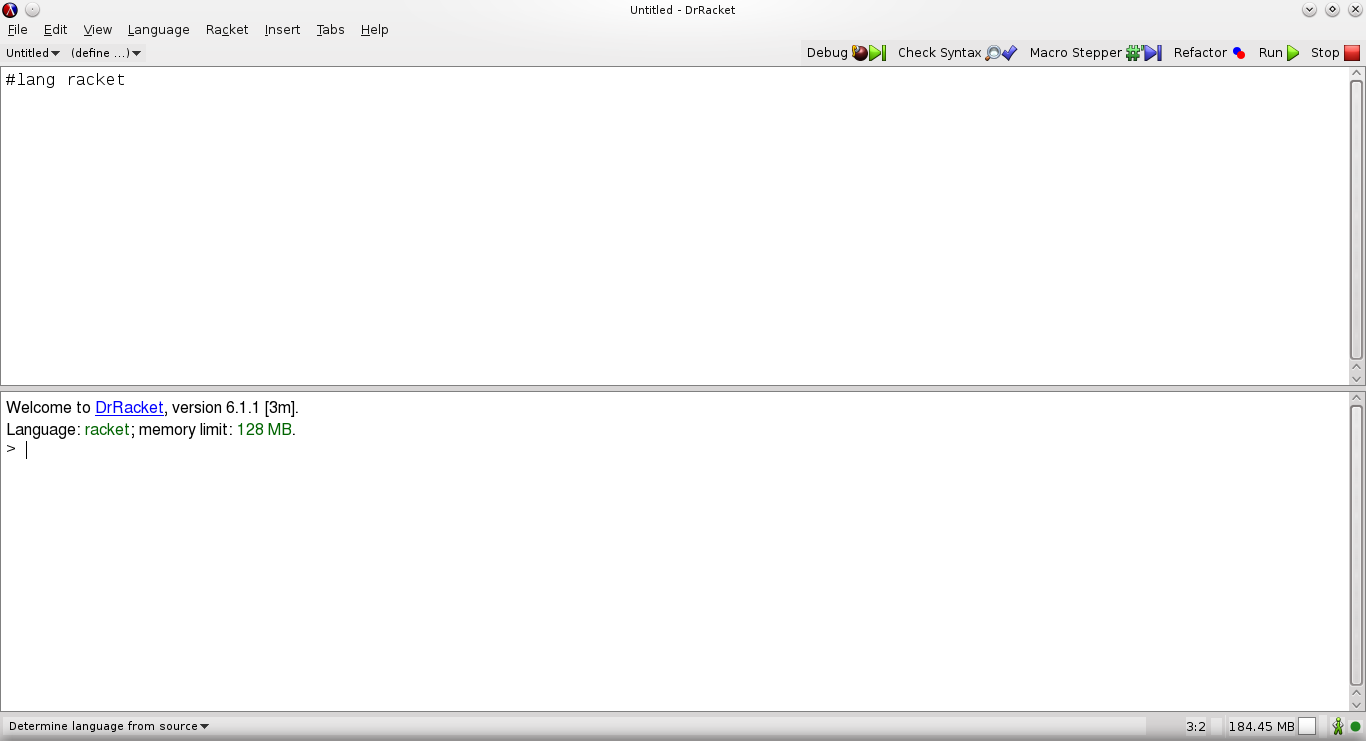
\includegraphics[width=1\textwidth]{img/DrRacketGui.png}
%	\caption{DrRacket Graphical user interface}
%	\label{fig:DrRacketGui}
%\end{figure}


%Base de dados preenchida durante a compilacao, que se presenta em forma de setas que eu vou usar para resolver os problemas semanticos.
%Seccao de critica/analise. 



%whereas Python is a very high-level programming language that supports the imperative, functional and object-oriented programming paradigms and is very popular in many areas.
The objective is to create a refactoring tool, for Racket in the DrRacket IDE, that helps and motivates unexperienced users to use refactoring operations. Racket is known for being used as an introductory programming course and DrRacket IDE is known as a pedagogic environment.

Besides being a simple and a good IDE to learn how to program, DrRacket gives some functionalities that are helpful to the programmer of the refactoring tool. 
DrRacket has a database filled during compile time that has information about all the bindings of each variable and DrRacket represents it in the visual form of arrows. 
Each arrow knows where is pointing to and where is the beginning of itself. 
This is rather helpful for the refactoring operations that need semantics.
For example, for the extract-function it makes it very easy to know what variables will be arguments of the extracted function and what variables are not needed to be passed as arguments.

DrRacket also has syntax objects. These objects have all the information regarding the syntactic information and their location. Basically they represent an annotated AST with the location of each object.

%By having this features it is possible to create a tool that helps the unexperienced users and it is useful for more experienced users.


